\documentclass{beamer}
\usetheme{Amurmaple}
\usepackage{graphicx}
\usepackage[table,xcdraw]{xcolor} % Allows for table coloring
\usepackage{colortbl} % Allows table border coloring
\usepackage{amsthm}
\usepackage{wrapfig}
\usepackage{multicol}
\usepackage{multirow}
\usepackage[dvipsnames]{xcolor}
\usepackage{ragged2e}
\usepackage{tikz}
% \usepackage{tikzpicture}
\usepackage{subcaption} % For subfigure environment
% \documentclass[tikz,border=2mm]{standalone}
\usetikzlibrary{arrows.meta,positioning}
\usetikzlibrary{shapes.geometric, positioning, backgrounds}



\title{Nash Equilibrium}
\subtitle{Part 2 \\Using Beamer}
\author{Arnab Sarker \& Enayet Alvee}
% \text {2105099  \& 2105107}
\institute{Bangladesh University of Engineering and Technology}
\date{\today}

\begin{document}

% Set page numbering to start from 28

\maketitle

\section{}
% \setcounter{page}{28} % Start from page 28

%part 2
\begin{frame}{Different Algorithms}
\setbeamercovered{transparent}
    \begin{itemize}
        \item<1> BruteForce
        \item<0> Exact Polynomial Algorithms
        \item<0> Approximation
    \end{itemize}
    
\end{frame}
% \setcounter{page}{28}

\begin{frame}{Different Algorithms: BruteForce}
\only<1-2>{
    \begin{center}
        \Large We can take all possible combinations of the supports for all players and check if it has reached a mixed nash equilibrium.
    \end{center}
    }
    \only<2>{
    But, \\
     \Large 
    \textcolor{red}{Number of combinations: }
    \begin{equation*}
      = \prod_{i=1}^{k}\left( 2^{M_i}-1\right)
    \end{equation*}
    \\
    {\small M = number of pure strategies available to a player \\
    k = number of players in the game.}
    }

    \only<3>{
    \begin{center}
            \Large But taking all the possible combinations will yield {\LARGE \textcolor{red}{ exponential time complexity}} !!
             \vspace{1cm}
        \begin{center}
            
\includegraphics[width=0.6\textwidth]{newimages/tiresomepic.png} % Replace 'path_to_image' with the actual path to your image
        \end{center}
    \end{center}
    }
\end{frame}

\begin{frame}{Different Algorithms}
\setbeamercovered{transparent}
    \begin{itemize}
        \item<0> BruteForce
        \item<1> Exact Polynomial Algorithms
        
        \item<0> Approximation
        
    \end{itemize}
    
\end{frame}


\begin{frame}{Exact Polynomial Algorithms}

    \begin{alertblock}
          \Large \textbf{Two-player Zero-Sum Games}
    \end{alertblock}


\only<1-6>{
    
      {\large A situation where \textcolor{ForestGreen}{one player's gain} is \textcolor{red}{the other player's loss}. \\ 
      The \textcolor{blue}{total gains and losses} of the players add up to \textbf{\textcolor{red}{zero.}}\\} 

      \only<1>{
        \vspace{1cm}
        \begin{center}
            
\includegraphics[width=0.6\textwidth]{newimages/2p0sum.png} % Replace 'path_to_image' with the actual path to your image
        \end{center}
      }

    
    \only<2-6>   
    % 
    {{Let's see an example :\\}
    \textcolor{red}{\large Rules: }\\
    }
    \begin{itemize}
        \only<2-6>    {\item Players have to raise either one or two fingers.}
        \only<3-6>   {\item Player 1 wins if the sum is \textbf{even}.}
        \only<4-6>    {\item Player 2 wins if the sum is \textbf{odd}.}
        \only<5-6>    {\item The winner gets \textbf{1} dollar from the loser.}
        \only<6>    {\item The sum of net winnings is \textbf{zero}.}
    \end{itemize}
}


\only<7-12>{
    \begin{table}[h]
    \centering
    \begin{tabular}{|c|c|c|c|}
    \hline
    \multicolumn{2}{|c|}{\textcolor{blue}{Raising Finger Game}} & \multicolumn{2}{c|}{Player 2} \\ \cline{3-4}
    \multicolumn{2}{|c|}{} & Strategy 1 & Strategy 2 \\ \hline
    \multirow{2}{*}{Player 1} 
    & Strategy 1 & \only<8-12>{1} & \only<9-12>{-1} \\ \cline{2-4}
    & Strategy 2 & \only<10-12>{-1} & \only<11-12>{1} \\ \hline
    \end{tabular}
    \caption{Payoff Matrix}
    \end{table}
}

\only<12>{
Expected payoff of player 1 = Expected loss of player 2
    \begin{wrapfigure}{l}{0.25\textwidth}
    \centering
    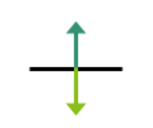
\includegraphics[width=0.20\textwidth]{Image/2p0sum.png}
    \end{wrapfigure}
    \textcolor{ForestGreen}{Player 1 Maximizes payoff} \\
    \textcolor{LimeGreen}{Player 2 Minimizes loss}  \\
}

\only<13>
   {\large  {For Two-Player-Zero-Sum games, finding a Nash equilibrium can often be done in \textbf{polynomial time} using \textit{linear programming methods.}\\}
    {Linear programs can be solved efficiently.}
    }
\end{frame}


\begin{frame}{Different Algorithms}
\setbeamercovered{transparent}
    \begin{itemize}
        \item<0> BruteForce
        \item<0> Exact Polynomial Algorithms
       
        \item<1> Approximation Algorithms
        
    \end{itemize}   
\end{frame}


\begin{frame}{Approximation Algorithms}

     \only<1->{
       \begin{alertblock}
          {\LARGE What is $\epsilon$-Nash equilibrium?}
      \end{alertblock}
     }
    \only<2>{
        {\Large \textcolor{blue}{Definition 1(Nash Equilibrium).}  }
    
        {A pair of strategies $(\hat{x}, \hat{y})$ is a Nash equilibrium for the bimatrix game $\Gamma = (A, B)$ if
        
        (i) For every (mixed) strategy $x$ of the row player, $x^T A \hat{y} \leq \hat{x}^T A \hat{y}$ and
        
        (ii) For every (mixed) strategy $y$ of the column player, $\hat{x}^T B y \leq \hat{x}^T B \hat{y}$.}
    
    }


    \only<3>{

        {\Large \textcolor{blue}{Definition 2($\epsilon$-Nash Equilibrium).}  }
        
        For any $\varepsilon > 0$, a pair of strategies $(\hat{x}, \hat{y})$ is an $\varepsilon$-Nash equilibrium for the bimatrix game $\Gamma = (A, B)$ if

        (i) For every (mixed) strategy $x$ of the row player, $x^T A \hat{y} \leq \hat{x}^T A \hat{y} + \varepsilon$, and
        
        (ii) For every (mixed) strategy $y$ of the column player, $\hat{x}^T B y \leq \hat{x}^T B \hat{y} + \varepsilon$.
    
    }
  
\end{frame}



\begin{frame}{$\epsilon$ Nash Equilibrium}
    \centering
    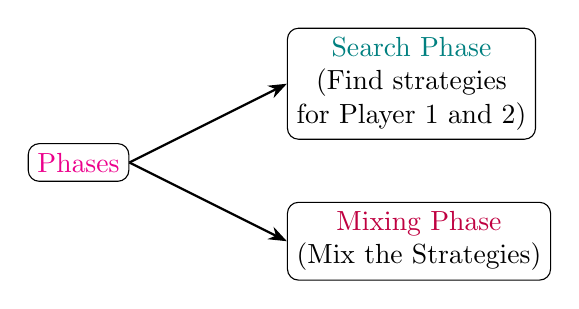
\begin{tikzpicture}[
        every node/.style={draw, align=center, rounded corners},
        arrow/.style={-{Stealth}, thick},
        node distance=2cm
    ]
    
    % Main Phase Node
    \node (main) {\textcolor{magenta}{Phases}};
    
    % Search Phase Node
    \node[right=of main, yshift=1cm] (search) {\textcolor{teal}{Search Phase} \\ (Find strategies \\ for Player 1 and 2)};
    
    % Mixing Phase Node
    \node[right=of main, yshift=-1cm] (mixing) {\textcolor{purple}{Mixing Phase} \\ (Mix the Strategies)};
    
    % Arrows
    \draw[arrow] (main.east) -- (search.west);
    \draw[arrow] (main.east) -- (mixing.west);
    
    \end{tikzpicture}

\end{frame}


%might be reducted

% \begin{frame}{$\frac{3}{4}$ - Nash Equilibrium}
%     \begin{lemma}
%         Consider any positively normalized $n*m$ bimatrix game $\Gamma=(A,B)$ and let $a_{i_1,j_1}$ = $\text{max}_{i,j}a_{i,j}$ and   $b_{i_2,j_2}$ = $\text{max}_{i,j}b_{i,j}$. Then the pair of strategies $(\hat{x},\hat{y})$ where $\hat{x_{i_1}}=\hat{x_{i_2}}=\hat{y_{i_1}}=\hat{y_{i_2}=\frac{1}{2}}$ is a $\frac{3}{4} $-Nash Equilibrium for $\Gamma$
%     \end{lemma}

%     \only<2>{
%     \begin{proof}
%         First observe that \\
%         \text{Expected payoff for player 1, } 
%         \begin{align*}
%             \hat{x}^T A \hat{y} &= \sum_{i=1}^n \sum_{j=1}^m \hat{x}_i \hat{y}_j a_{i,j} \\
%             &= \hat{x}_{i_1} \hat{y}_{j_1} a_{i_1,j_1} +  \hat{x}_{i_1} \hat{y}_{j_2} a_{i_1,j_2} +  \hat{x}_{i_2} \hat{y}_{j_1} a_{i_2,j_1} +  \hat{x}_{i_2} \hat{y}_{j_2} a_{i_2,j_2} \\
%             &= \frac{1}{4}(a_{i_1,j_1} + a_{i_1,j_2} + a_{i_2,j_1}+ a_{i_2,j_2}) \\
%             &\geq \frac{1}{4} a_{i_1,j_1}.
%         \end{align*}
%     \end{proof}
%     }
%     \only<3>{
%    \begin{proof}
%         Similarly
%         \text{Expected payoff for player 2, } 
%         \begin{align*}
%             \hat{x}^T B \hat{y} &= \sum_{i=1}^n \sum_{j=1}^m \hat{x}_i \hat{y}_j b_{i,j} \\
%             &= \hat{x}_{i_1} \hat{y}_{j_1} b_{i_1,j_1} +  \hat{x}_{i_1} \hat{y}_{j_2} b_{i_1,j_2} +  \hat{x}_{i_2} \hat{y}_{j_1} b_{i_2,j_1} +  \hat{x}_{i_2} \hat{y}_{j_2} b_{i_2,j_2} \\
%             &= \frac{1}{4}(b_{i_1,j_1} + b_{i_1,j_2} + b_{i_2,j_1}+ b_{i_2,j_2}) \\
%             &\geq \frac{1}{4} b_{i_1,j_1}.
%         \end{align*}
%     \end{proof}
%     }
    
%     \only<4>{
%     \begin{proof}
%          Now observe that, for any (mixed) strategies $x \text { and } y$ of the player 1 \& 2 respectively, 
%         \begin{equation*}
%              x^T A \hat{y} \leq  a_{i_1,j_1}  \text{ and }   \hat{x}^T B \hat{y} \leq  b_{i_2,j_2}
%         \end{equation*}
%         and recall that  $a_{i,j}$ $\epsilon$  $[0,1]$ for all 
%         $i\text{ } \epsilon\text{ } N \text{ , } j \text{ } \epsilon \text{ } M.$ Hence 
%         \begin{equation*}
%             x^T A \hat{y} \leq  a_{i_1,j_1}=\frac{1}{4}a_{i_1,j_1}+\frac{3}{4}a_{i_1,j_1}  \leq   \hat{x}^T A \hat{y} + \frac{3}{4}
%         \end{equation*}
%     \end{proof}
%     }



%     \only<5>{
%     {
%     \begin{proof}
%         and,
%         \begin{equation*}
%                 \hat{x}^T B \hat{y} \leq  b_{i_2,j_2}=\frac{1}{4}b_{i_2,j_2}+\frac{3}{4}a_{i_2,j_2} \leq   x^T B \hat{y} + \frac{3}{4}
%         \end{equation*}
        
%     \end{proof}
%     }
%     Thus \textbf{$(\hat{x},\hat{y})$} is a $\frac{3}{4}$ -Nash equillibrium for $\Gamma$.
        
%   }      
    
% \end{frame}


\begin{frame}{Time Complexeties of $\epsilon$ -Nash Equilibrium}
   % \setbeamercovered{transparent}
    \begin{table}[ht]
    \centering
    \renewcommand{\arraystretch}{1.5} % Adjust row height
    \begin{tabular}{|p{3.2cm}|p{1.2cm}|p{1.3cm}|p{2cm}|p{1.5cm}|}
        \hline
        {\textbf{Name} & \textbf{Bound proven by original papers} & \textbf{Bound computed from programs} & \textbf{Time complexity} & \textbf{Running time from programs (sec)}} \\
        \hline
        \only<1->{$\frac{3}{4}$ - Nash equilibrium for bimatrix game} & \only<1-> {0.75} & \only<1->{0.75} & \only<1->{$O(mn)$} & \only<1->{1.39} \\
        \hline
        \only<2->{$\frac{1}{2}$ - Nash equilibrium for bimatrix game} & \only<2-> {0.5} & \only<2->{0.5} & \only<2->{$O(mn)$} & \only<2->{0.06} \\
        \hline
        \only<3->{$\frac{(3-\sqrt{5})}{2}$ - Nash equilibrium for bimatrix game} & \only<3->{{\small 0.381966}} & \only<3->{{\small 0.381966}} & \only<3->{Polynomial time} & \only<3>{4.63} \\
        \hline
    \end{tabular}
    \caption{Table of Results}
    \end{table}

   
\end{frame}

% \begin{frame}{Metaheuristic Algorithms}
    
% \end{frame}

% \begin{frame}{summarization}
%     \begin{table}[ht]
%     \centering
%     \caption{Metaheuristics Algorithms Summarized}
%     \begin{tabular}
%     {|p{2.5cm}|p{6cm}|p{2.5cm}|}
%     \hline
%     \textbf{Algorithm Name} & \textbf{Short Description} & \textbf{Per Iteration Complexity} \\
%     \hline
%     \textbf{Replicator Dynamics} & {\small Evolutionary algorithm where players' strategies evolve over time based on payoff ratios, imitating more successful strategies.} & $O(N^2)$ \\
%     \hline
%     {\small \textbf{Particle Swarm Optimization (PSO)}} & {\small Population-based optimization algorithm where particles represent strategy profiles. They iteratively update based on personal and global best solutions.} & $O(PNK)$ \\
%     \hline
%     \textbf{Simulated Annealing (SA) }& {\small A single-point optimization technique that probabilistically explores the strategy space, reducing the search range over time.} & $O(NK)$ \\
%     \hline
%     \end{tabular}
%     \end{table}
% \end{frame}
    
% \begin{frame}{Metaheuristics Algorithm summarized}
%     P = number of particles/solutions in population-based algorithms \\
%     N = number of players \\
%     K = number of strategies available to a player    
% \end{frame}
    

% \begin{frame}{Heuristic Algorithms}
    
% \end{frame}


% \begin{frame}{heuristics Algorithm Summarized}
  
%     \begin{table}[ht]
%     \centering
%     \caption{Metaheuristics Algorithms Summarized}
%     \begin{tabular}
%     {|p{2.5cm}|p{6cm}|p{2.5cm}|}
%     \hline
%     \textbf{Algorithm Name} & \textbf{Short Description} & \textbf{Per Iteration Complexity} \\
%     \hline
%     \textbf{Local Search
%     } & {\small Iteratively improves a solution by exploring neighboring solutions and accepting better ones.
%     } &$O(NK)$  \\
%     \hline
%     {\small \textbf{Best Response Dynamics}} & {\small Players iteratively choose their best response (greedy choice) given the current strategies of others.
%     } & $O(NK)$  \\
%     \hline
%     \textbf{Hill Climbing}& {\small A greedy algorithm that moves to the best neighboring solution, but may get stuck in local optima.
%     } & $O(NK)$ \\
%     \hline
%     \end{tabular}
%     \end{table}

    
    
% \end{frame}
    



\begin{frame}{Applications}
    \begin{figure}[h]
    \centering
    
\includegraphics[width=0.7\textwidth]{newimages/application.png}
    \caption{Applications of Nash Equilibrium}
\end{figure}
\end{frame}



\begin{frame}{Theoretical Application}
    \begin{figure}[h]
        \centering
        \begin{subfigure}[b]{0.3\textwidth}
            
\includegraphics[width=\textwidth]{Image/GameLudu.png}
            \caption{\textcolor{red}{\\Game Theory Analysis}\\
            Nash Equilibrium is used to predict and analyze the outcomes of strategic games.}
        \end{subfigure}
        \hfill
        \begin{subfigure}[b]{0.3\textwidth}
            
\includegraphics[width=\textwidth]{Image/Economic.png}
            \caption{\textcolor{blue}{\\Economic Models}\\Nash Equilibrium is used to analyze oligopolistic markets, bidders’ behaviors in auctions etc. }
        \end{subfigure}
        \hfill
        \begin{subfigure}[b]{0.3\textwidth}
            
\includegraphics[width=\textwidth]{Image/biology virus.png}
             % \vspace{2cm}
            \caption{\textcolor{BurntOrange}{\\
            Biology and Evolution}\\Nash Equilibrium helps to understand competition and cooperation strategies among species populations.}
        \end{subfigure}
    \end{figure}
\end{frame}

\begin{frame}{Applications of Nash Equilibrium}
\begin{tikzpicture}[node distance=1.cm and 1.2cm, font=\small]  % Reduced node distance and font size

    % Central node
    \node (nash) [circle, draw=black, fill=yellow!50, text centered, minimum size=2cm, thick, font=\bfseries] {Nash \\ Equilibrium};
    
    % Outer nodes
    \only<2->{\node (economics) [rectangle, rounded corners, draw=black!70, fill=blue!10, text width=2.5cm, text centered, minimum height=1cm, above=of nash] {\textbf{Economics} \\ Pricing strategies for stability.};}
    \only<8->{\node (traffic) [rectangle, rounded corners, draw=black!70, fill=blue!10, text width=2.5cm, text centered, minimum height=1cm, left=of nash] {\textbf{Traffic} \\ Shortest travel routes.};}
    \only<5->{\node (politics) [rectangle, rounded corners, draw=black!70, fill=blue!10, text width=3cm, text centered, minimum height=1cm, below right=of nash] {\textbf{Politics} \\ Candidate strategies stabilize votes.};}
   \only<4->{ \node (sports) [rectangle, rounded corners, draw=black!70, fill=blue!10, text width=2.5cm, text centered, minimum height=1cm, right=of nash] {\textbf{Sports} \\ Balancing strategies for advantage.};}
    \only<3->{\node (ecommerce) [rectangle, rounded corners, draw=black!70, fill=blue!10, text width=2.5cm, text centered, minimum height=1cm, above right=of nash] {\textbf{E-Commerce} \\ Optimizing discounts for margins.};}
    \only<1->{\node (socialmedia) [rectangle, rounded corners, draw=black!70, fill=blue!10, text width=2.5cm, text centered, minimum height=1cm, above left=of nash] {\textbf{Social Media} \\ Optimizing content for engagement.}};
    \only<7->{\node (machinelearning) [rectangle, rounded corners, draw=black!70, fill=blue!10, text width=3cm, text centered, minimum height=1cm, below left=of nash] {\textbf{Machine Learning} \\ Algorithms optimize predictions.}};
    \only<6->{\node (healthcare) [rectangle, rounded corners, draw=black!70, fill=blue!10, text width=3.5cm, text centered, minimum height=.5cm, below =of nash] {\textbf{Healthcare }\\ Treatment strategies balance cost and effectiveness.};}



    % Connections
    \only<2->{\draw[->, thick, draw=black!70] (nash) -- (economics);}
    \only<8->{\draw[->, thick, draw=black!70] (nash) -- (traffic);}
    \only<5->{\draw[->, thick, draw=black!70] (nash) -- (politics);}
    \only<4->{\draw[->, thick, draw=black!70] (nash) -- (sports);}
    \only<3->{\draw[->, thick, draw=black!70] (nash) -- (ecommerce);}
    \only<1->{\draw[->, thick, draw=black!70] (nash) -- (socialmedia);}
    \only<7->{\draw[->, thick, draw=black!70] (nash) -- (machinelearning);}
    \only<6->{\draw[->, thick, draw=black!70] (nash) -- (healthcare);}
    
    % Optional: Add background for clarity
    % \begin{scope}[on background layer]
    %     \fill[blue!5] ($(nash)+(-3,-3)$) rectangle ($(nash)+(3,3)$);
    % \end{scope}

\end{tikzpicture}
\end{frame}


\begin{frame}{Real Life Examples}

    \begin{center}
        \begin{tcolorbox}[
            colback=blue!5!white,
            colframe=blue!75!black,
            width=0.8\textwidth,
            boxrule=1mm,
            sharp corners,
            fonttitle=\bfseries,
            title=Quote by Albert Einstein
        ]
            \begin{minipage}[c]{0.3\textwidth}
                
\includegraphics[width=\textwidth]{newimages/einstein.png} % Replace with your image file
            \end{minipage}
            \hfill
            \begin{minipage}[c]{0.65\textwidth}
                \centering
                \textit{"Life is just like a game, \\
                First you have to learn rules of the game, \\
                And then play it better than anyone else."} \\[0.3cm]
                \textbf{- Albert Einstein}
            \end{minipage}
        \end{tcolorbox}
    \end{center}
     
\end{frame}


\begin{frame}{Real Life Applications}

% Title with color and formatting


\vspace{0.5cm} % Adds space after title for better readability

\noindent
\begin{minipage}[t]{0.7\textwidth} % Text block on the left
    \justifying % Justified text
    {\Large \textcolor{blue}{\textbf{Sports:\\}}}
    \begin{itemize}
        \only<1->{\item {\large Teams must decide on their strategies in competitive sports.}}

     \only<2->{\item {\large For example, football teams need to choose defensive, attacking, or neutral strategies in response to the opponents’ strategies.}}

      \only<3->{ \item {\large Too much defensive or too much attacking strategy may result in severe failure.}}
    \end{itemize}
\end{minipage}%
\hfill
\begin{minipage}[t]{0.25\textwidth} % Images block on the right
    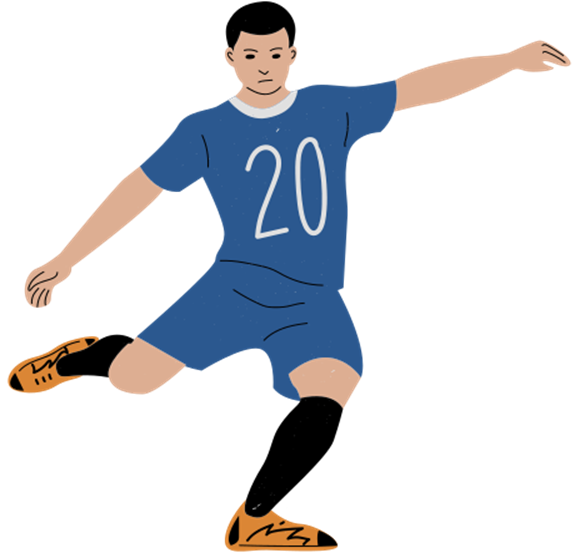
\includegraphics[width=\textwidth]{newimages/image_footballer.png} % Replace with your first image
    \vspace{1cm} % Adds space between images
    
\includegraphics[width=.7cm]{newimages/football.png} % Replace with your second image
\end{minipage}

\end{frame}





\begin{frame}{Real Life Application}
    % Title styling
    \begin{tcolorbox}[colback=white, colframe=white, boxrule=0pt, top=0pt, bottom=0pt, left=0pt, right=0pt, width=\textwidth, sharp corners]
        \textcolor{red}{\LARGE \textbf{Price Wars}}
    \end{tcolorbox}
    
    % Content
    \justifying
    \textbf{
        \begin{itemize}
           \only<1->{ \item In highly competitive markets, companies often engage in price wars to gain market share and attract customers.}
         \only<2->{\item Controlling the supply in the market allows companies to influence prices to rise.}
          \only<3->{  \item Competitors can attract more customers by cutting prices.}
        \end{itemize}
    }
    
    % Insert image
    \begin{figure}[h]
        \centering
        
\includegraphics[width=0.3\textwidth]{newimages/moneybag.png}
        
\includegraphics[width=.2\textwidth]{newimages/money.png}% Replace with your actual file path
    \end{figure}
\end{frame}

\begin{frame}{}
  \centering
  \emph{\LARGE THANK YOU}
\end{frame}

   

\end{document}
